\documentclass{article}

\usepackage{minitoc}
\usepackage{tabularx}
\usepackage{booktabs}
\usepackage{graphicx}
\usepackage{hyperref}
\usepackage{xcolor}
\usepackage{blkarray}
\usepackage{amsthm, amssymb, amsmath}
\usepackage{caption}
\usepackage{subcaption}
\usepackage{multirow}
\usepackage[ruled,vlined]{algorithm2e}

\usepackage{natbib}
\bibliographystyle{abbrvnat}

\theoremstyle{definition}
\newtheorem{definition}{Definition}[section]
\newtheorem{theorem}{Theorem}[section]
\newtheorem{lemma}[theorem]{Lemma}
\newtheorem{conjecture}[theorem]{Conjecture}
\newtheorem{corollary}{Corollary}[theorem]

\usepackage[margin=2.5cm, includefoot, footskip=30pt]{geometry}
\pagestyle{plain}
\setlength{\parindent}{0em}
\setlength{\parskip}{1em}

\renewcommand{\baselinestretch}{1}

\usepackage{standalone}

\newtheorem{proposition}{Proposition}

\title{$n-$bits reactive strategies}

\author{Nikoleta E. Glynatsi, Ethan Akin, Martin Nowak, Christian Hilbe}
\date{}

\begin{document}

\maketitle

\begin{abstract}

We focus on repeated games and the strategies players can employ in these
games. It is famously assumed in repeated games that strategies utilizing past
history can be employed. Here, we concentrate on a specific set of strategies
known as reactive strategies. Notably, our work stands out by exploring
strategies with longer memory spans, in contrast to the prevailing norm in
existing literature.

We demonstrate, how this set of strategies have an imidate effect
of the co-oplayer and show that a history that is not shared does not befenit
the longer strategy.


In the following we study repeated games and the strategies player's can
derive in these games. Famously, in repeated game it is assumed that strategies
that use the past history can be adopted. Here we focus on such a set, called the
reactive strategies. In comparison to previous studies this work explores higher
memory strategies, greater than one compared to the majority of the works in the
literature. We demonstrate, how this set of strategies have an imidate effect
of the co-oplayer and show that a history that is not shared does not befenit
the longer strategy.

We then characterise partner strategies, which are strategies assuring mutual
cooperation without being exploited. A recipe for evolutionary stability.
We show that the class of Tit For Tat and Generous Tit For strategies even the
delayed versions of these strategies are partner strategies.

For memory lengths of two and three we characterize all partner strategies
amongst the reactive set. The conditions simple and yet newly found. For a specific
class of reactive counting strategies, counting of defections/defections instead
of remembering the actual occurance of the action, we can characterize partner
strategies in all memory lengths.

We further test the evolutionary properties of partner strategies in higher memory.
The results show that.

\end{abstract}

\section{Introduction}

\section{Model}

We consider an infinitely repeated game with two players. In each round, player 1
and player 2, can choose to cooperate ($C$) or to defect ($D$). If both players
cooperate, they receive a payoff $R$ (the reward for mutual cooperation), and if
both players defect, they receive a payoff $P$ (the punishment for mutual
defection). If one player cooperates, the cooperative player receives the
sucker's payoff $S$, and the defecting player receives the temptation payoff
$T$. We assume that the payoff are such that $T > R > P > S$ and $2 R > T + S$.
This game is known as the Prisoner's Dilemma. Here, we
employ a specific parametrization of the Prisoner's Dilemma, where cooperation
implies incurring a cost $c$ for the co-player to derive a benefit $b > c$.
Consequently, the payoffs are defined as follows: \(R = b - c, S = -c, T = b, P =
0\). In the Appendix, we present results applicable to the general Prisoner's
Dilemma.

We assume in the following, that the players' decisions only depend on the
outcome of the previous $n$ rounds. To this end, an {\it $n$-history for player
$i \in \{1, 2\}$} is a string $h^i=(a^i_{-n},\ldots,a^i_{-1})\!\in\!\{C,D\}^n$
where an entry $a^i_{-k}$ corresponds to player $i$'s action $k$ rounds ago. Let
$H^i$ denote the space of all $n$-histories for player $i$ where set $H^i$ contains
$|H^i|=2^{n}$ elements. A {\it reactive$-n$ strategy} for player 1 is a vector
$\mathbf{p}=(p_h)_{h\in H^2} \in [0, 1]^{n}$. Each entry $p_h$ corresponds to
the player's cooperation probability in the next round, based on the co-player's
actions in the previous $n$ rounds. Therefore, reactive-$n$ strategies
exclusively rely on the co-player's $n$-history, independent of the focal
player's own actions. For \(n=1\), this definition of reactive-\(n\) strategies
recovers the typical format of reactive-1 strategies~\citep{baek:scientific:2016, wahl:JTB:1999, mcavoy:PRSA:2019},
\(\mathbf{p}=(p_C, p_D,)\).

Another class of strategies we will be discussing in this work are, {\it
self-reactive-$n$} strategies which only consider the focal player's own
$n$-history, and ignore the co-player's. Formally, a self-reactive-$n$ strategy
for player 1 is a vector $\mathbf{\tilde{p}} = (\tilde{p}_h)_{h \in H^1} \in [0,
1] ^ {n}$. Each entry $\tilde{p}_h$ corresponds to the player's cooperation
probability in the next, depending on the player's own actions in the previous
$n$ rounds. We say that a reactive or self-reactive strategy is pure if all the
entries of the strategy are either 0 or 1. We refer to the set of all pure
self-reactive strategies as $\tilde{P}_n$.

\begin{figure}[h!]
  \centering
  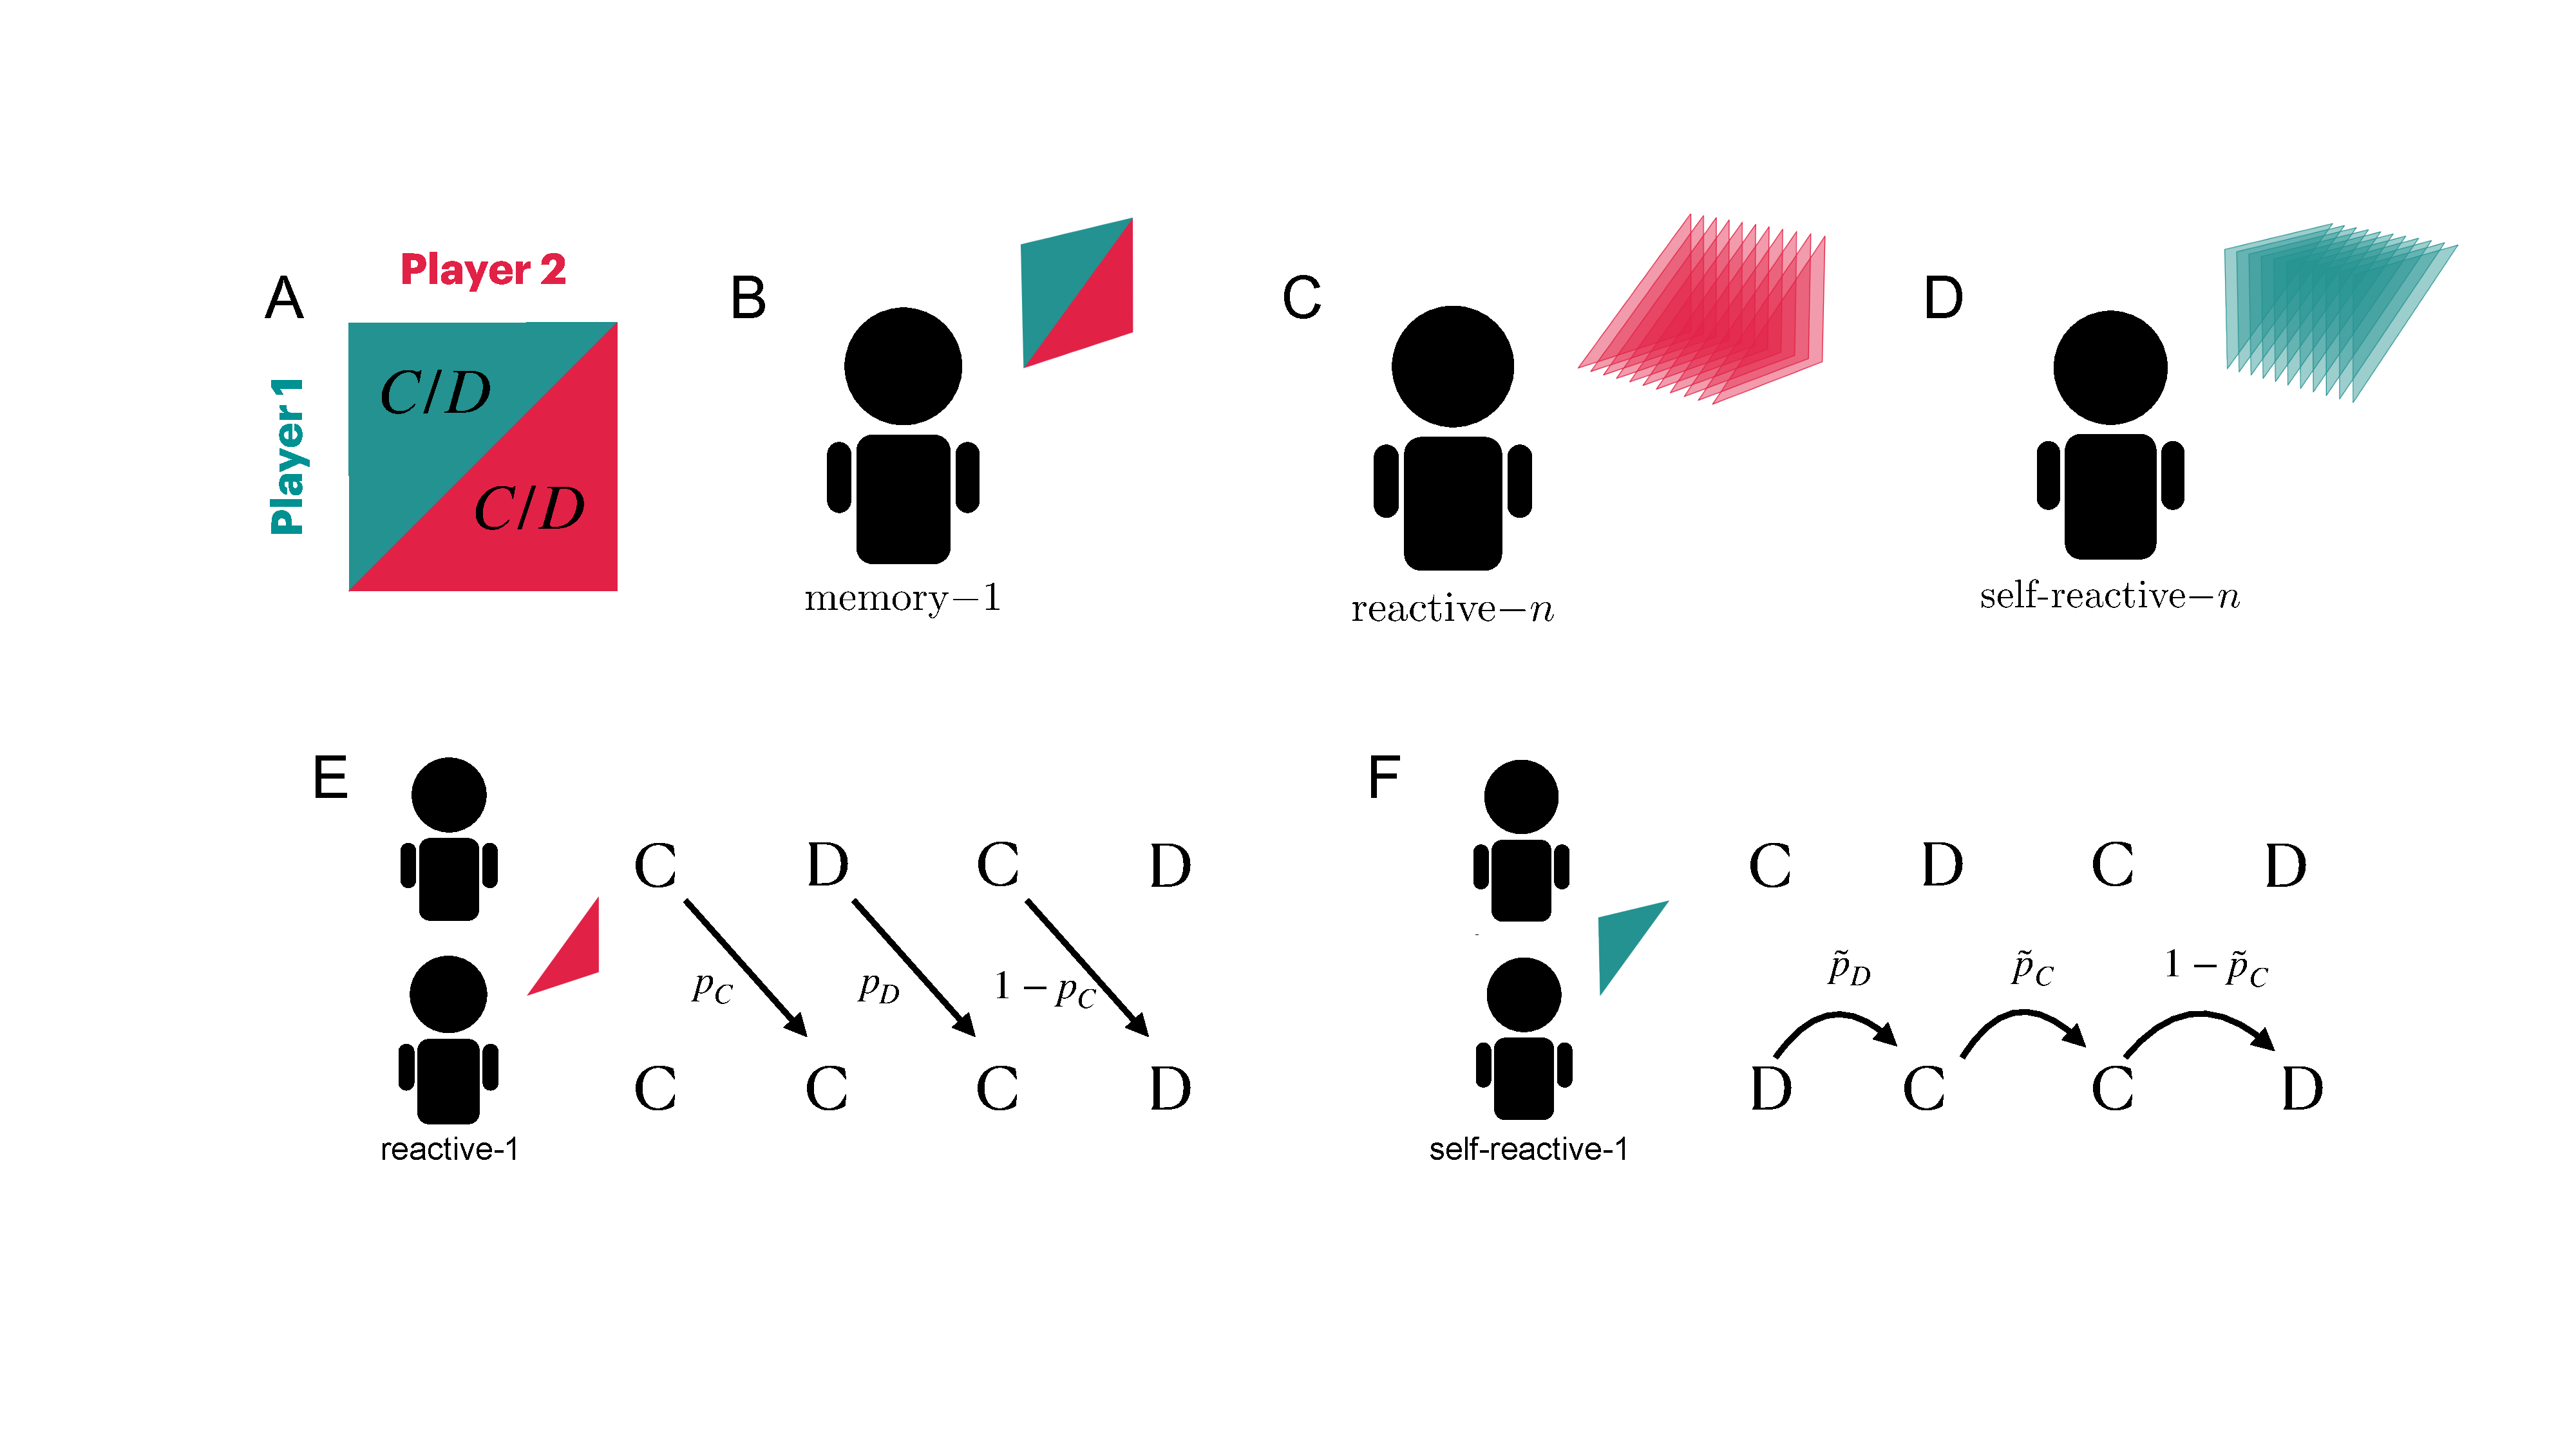
\includegraphics[width=\textwidth]{figures/conceptual_figure_model.pdf}
  \caption{\textbf{Model.}
  \textbf{A.} In each turn of the repeated game, players 1 and 2 decide on an action,
  denoted as $C$ (cooperate) or $D$ (defect), respectively. We assume, that the information that a
  player can use in subsequent turns is limited to the actions taken by both
  players in the current turn.
  \textbf{B.} Memory-$1$ strategies, a well-studied set of strategies, utilize the
  actions of both players in the previous turn to make decisions. In the graphical
  representation of memory-$1$ strategies, we use a single square to illustrate this
  concept.
  \textbf{C.} This work primarily focuses on reactive-$n$ strategies, which take
  into account only the actions of the co-players.
  \textbf{E.} For the case of $n = 1$, a reactive-$1$ strategy is represented as a vector $\mathbf{p} =
  (p_C, p_D)$, where $p_C$ is the probability of cooperating given that the co-player
  cooperated, and $p_D$ is the probability of cooperating given that the co-player
  defected. In the example shown, the bottom player employs a reactive-$1$ strategy.
  They cooperate with a probability $p_C$ in the second round because the co-player
  cooperated in the first round. In the second round, the player cooperates with a
  probability pD since the co-player previously defected. Finally, the player
  defects in the third round with a probability of $1 - p_C$, considering that the
  co-player cooperated.
  \textbf{D.} Another set of strategies we consider is that of self-reactive-$n$
  strategies, which rely solely on a player's own previous $n$ actions.
  \textbf{F.} For the case of $n = 1$, a self-reactive-$1$ strategy is represented
  as a vector $\mathbf{\tilde{p}} = (\tilde{p}_C, \tilde{p}_D)$, where
  $\tilde{p}_C$ is the probability of cooperating given that the player's last
  action was cooperation, and $\tilde{p}_D$ is the probability of cooperating
  given that the player's last action was defection. In the example shown, the
  bottom player employs a self-reactive-$1$ strategy. They cooperate with a
  probability $\tilde{p}_D$ in the second round given that they defected in the
  first. In the second round, the player cooperates with a probability
  $\tilde{p}_C$ since they cooperated in the previous round. Finally, the player
  defects in the third round with a probability of $1 - \tilde{p}_C$, considering
  that they cooperated in the previous round.}
\end{figure}

\section{Results}

\subsection{Self-Reactive Sufficiency}

To predict which reactive-$n$ strategies are partner strategies, we must first
characterize which nice reactive-$n$ strategies are Nash equilibria. Determining
whether a given strategy, $\mathbf{p}$, is a Nash equilibrium is not
straightforward. In principle, this would involve comparing the payoff of
$\mathbf{p}$ to the payoff of all possible mutant strategies. However, in this
work, we demonstrate otherwise. Specifically, we show that if a player adopts a
reactive strategy, it is only necessary to consider mutant strategies that are
self-reactive-$n$. In other words, we show the following result (see Appendix for
proof),

\begin{lemma}\label{lemma:self_reactive_sufficiency}
  Let $\mathbf{p}$ be a reactive$-n$ strategy for player $1$. Then, for any
  memory$-n$ strategy $\mathbf{m}$ used by player $2$, player $1$'s score is
  exactly the same as if $2$ had played a specific self-reactive memory-$n$
  strategy $\mathbf{\tilde{p}}$.
\end{lemma}

Our result aligns with the findings of~\citep{press:PNAS:2012}. They explored a
scenario where one player uses a memory-1 strategy while the other employs a
longer memory strategy. They demonstrated that the payoff of the player with the
longer memory is exactly the same as if they had used a specific shorter-memory
strategy, disregarding any history beyond what is shared with the short-memory
player. Our results hint at a more general insight: if one player does not
observe a part of the history, the co-player gains no advantage by considering
the unshared history.

Lemma~\ref{lemma:self_reactive_sufficiency} allows us to focus on self-reactive
strategies when evaluating whether a reactive strategy is a Nash equilibrium.
This significantly reduces the search space for potential mutants. Our next
result further reduces this space:

\begin{lemma}\label{lemma:nash_against_pure_self_reactive}
  A reactive-$n$ strategy $\mathbf{p}$, is a \textit{Nash strategy} if,

  \begin{equation}\label{Eq:NashReactive}
      s_{\mathbf{\tilde{p}}, \mathbf{p}} \leq s_{\mathbf{p},\mathbf{p}} \;\forall \; \tilde{p} \in \tilde{P}.
  \end{equation}
\end{lemma}

See Appendix for proof.

In the case of $n=3$ there are are $2^8 = 256$ possible self-reactive strategies.
As opposed to memory-3 strategies where there are $2^8 \times 2^8 = 65536$. Thus,
the number of strategies we need to check against is reduced by a factor of 256.

\subsection{Partner Strategies Amongst Reactive-2 and Reactive-3 Strategies}

Previous studies have characterized subsets of partner strategies for $n = 2$,
and while we also focus on characterizing a subset, our contribution extends to
the complete set of reactive-$2$ strategies. Furthermore, we extend the analysis
to the case of $n = 3$. We begin by characterizing partner strategies amongst
the set of reactive-$2$.

\begin{theorem}[``Reactive-2 Partner Strategies'']\label{theorem:reactive_two_partner_strategies}
A nice reactive-two strategy $\mathbf{p}$, is a partner strategy if and only if,
the strategy entries satisfy the conditions:

\begin{equation}\label{eq:two_bit_conditions}
  \displaystyle p_{DD} < 1\!-\! \frac{c}{b}  ~~and~~ \displaystyle \frac{p_{CD} + p_{DC}}{2} < 1- \frac{1}{2} \cdot \frac{c}{b}.
\end{equation}
\end{theorem}

These conditions can be summarized as follows: For the strategy to be Nash, the
strategy ALLD must not be able to invade ($p_{DD} \leq 1 - \frac{c}{b}$
ensures this), and the average cooperation rate following a defection must be
less than half of the cost-benefit ratio ($c/b$).

We can characterizing partner strategies amongst
the set of reactive-$3$. In the case of $n=3$, a nice reactive-3 strategy is
given by a vector

$$\mathbf{p}=(p_{CCC}, p_{CCD}, p_{CDC}, p_{CDD}, p_{DCC}, p_{DCD}, p_{DDC}, p_{DDD}).$$

\begin{theorem}[``Reactive-Three Partner Strategies'']\label{theorem:reactive_three_partner_strategies}
  A nice reactive-three strategy $\mathbf{p}$, is a partner strategy if and only if,
  the strategy entries satisfy the conditions:
  
  \begin{align}\label{eq:three_bit_conditions}
    \begin{split}
    p_{DDD} & < 1\!-\! \frac{c}{b} \\
    \frac{p_{CCD} + p_{CDC} + p_{DCC}}{3} & < 1\!-\! \frac{1}{3} \cdot \frac{c}{b} \\
    \frac{p_{CDD} + p_{DCD} + p_{DDC}}{3} & < 1\!-\! \frac{2}{3} \cdot \frac{c}{b} \\
    \frac{p_{CCD} + p_{CDD} + p_{DCC} + p_{DDC}}{4}  & < 1\!-\! \frac{1}{2} \cdot \frac{c}{b}  \\
    \frac{p_{CDC} + p_{DCD}}{2} & < 1\!-\! \frac{1}{2} \cdot \frac{c}{b}
    \end{split}
  \end{align}
\end{theorem}

Increasing the memory we allow strategies by one results to five conditions instead
of two. Inherently, these conditions still exhibit some symmetry with the
previous case. The strategy should not be invaded by the strategy ALLD,
resulting in the condition $p_{DDD} < 1 - \frac{c}{b}$. Additionally, the
average cooperation following a single defection must be lower than 2/3 of the
cost-benefit ratio, and the average cooperation following two defections must be
smaller than 1/3 of the cost-benefit ratio. There are two additional conditions
that do not appear to have clear interpretations. We hypothesize that as the
memory space we allow increases, the number of conditions will also increase,
and some of the conditions will deviate from the symmetry.

The proofs for both theorems can be found in the Appendix. We can prove the
results of this in two independent ways. One leverages the findings of Lemma
3.2, where we explicitly derive the payoff expressions against all pure
self-reactive strategies. The second method utilizes the techniques and results
presented in [Akin, 2016]. In the Appendix, we demonstrate how one of the
central results from Akin's work can be generalized.


\subsection{Partner Strategies Amongst Reactive Counting Strategies}

A special case of reactive strategies is reactive counting strategies. These are
strategies that respond to the co-player's actions, but they do not distinguish
between when cooperations/defections occurred; they solely consider the count of
cooperations in the last $n$ turns. A reactive-$n$ counting strategy is represented
by a vector $\mathbf{r}=(r_i)_{i \in \{n, n -1, \dots, 0\}}$, where the entry \(r_i\)
indicates the probability of cooperating given that the co-player cooperated
\(i\) times in the last \(n\) turns.

Reactive-two counting strategies are denoted by the vector $\mathbf{r}=(r_2,
r_1, r_0)$. We can characterise partner strategies among the reactive-two
counting strategies by setting $r_2 = 1$, and $p_{CD} = p_{DC} = r_1$ and
$p_{DD} = r_0$ in conditions~\eqref{eq:two_bit_conditions}. This gives us the
following result.

\begin{corollary}
A nice reactive-two counting strategy $\mathbf{r} = (1, r_1, r_0)$ is a partner strategy if and only if,

\begin{equation}\label{eq:counting_two_bit_conditions}
  \displaystyle r_1 < 1-\frac{1}{2} \cdot \frac{c}{b} ~~and~~ r_0 < 1\!-\! \frac{c}{b}.
\end{equation}
\end{corollary}

Reactive-three counting strategies are denoted by the vector $\mathbf{r}=(r_3,
r_2, r_1, r_0)$. We can characterise partner strategies among reactive-three
counting strategies by setting $r_3 = 1$, and $p_{CCD} = p_{CDC} = p_{DCC} =
r_2, p_{DCD} = p_{DDC} = p_{CDD} = r_1$ and $p_{DDD} = r_0$ in
conditions~\eqref{eq:three_bit_conditions}. This gives us the following result.

\begin{corollary}
A nice reactive-three counting strategy $\mathbf{r} = (1, r_2, r_1, r_0)$ is a partner strategy if and only if,

\begin{equation}\label{eq:counting_three_bit_conditions}
  \displaystyle r_2 < 1- \frac{1}{3} \cdot \frac{c}{b}, \quad r_1 < 1- \frac{2}{3} \cdot \frac{c}{b} ~~and~~ r_0 < 1\!-\! \frac{c}{b}.
\end{equation}
\end{corollary}

In the case of reactive-1 strategies, counting strategies are equivalent.
Howver, even in the case of reactive-2 strategies the conditions do not changes.
The ratio has to be smaller than. It's the the case of reactive-3 strategies
that we observe the biggest difference. That is the are three conditions instead
of five. The top conditions we can not account for are the conditions.

The properties of the reactive counting strategies are interesting. They allow
us to character partner strategies in all memory lengths.

\begin{corollary}[``Reactive-Counting Partner Strategies'']\label{corollary:reactive_counting_partner_strategies}
A nice reactive-$n$ counting strategy $\mathbf{r}$,
is a partner strategy if and only if:

\begin{equation}
  r_{n - k} < 1 - \frac{k}{n} \cdot \frac{c}{b}, \text{ for } k \in \{1, 2, \dots, n\}.
\end{equation}
\end{corollary}

Regadless of the memory length, the conditions are the same. The ratio has to be
smaller than the franction of benefit and the tolerence or otherwise, the
fogivmess which is measure by a higher propability of coopeariong given a
defection, decreases as the number of defections by the co-player increase. 


\subsection{Evolutionary Dynamics}

\begin{figure}[h!]
  \centering
  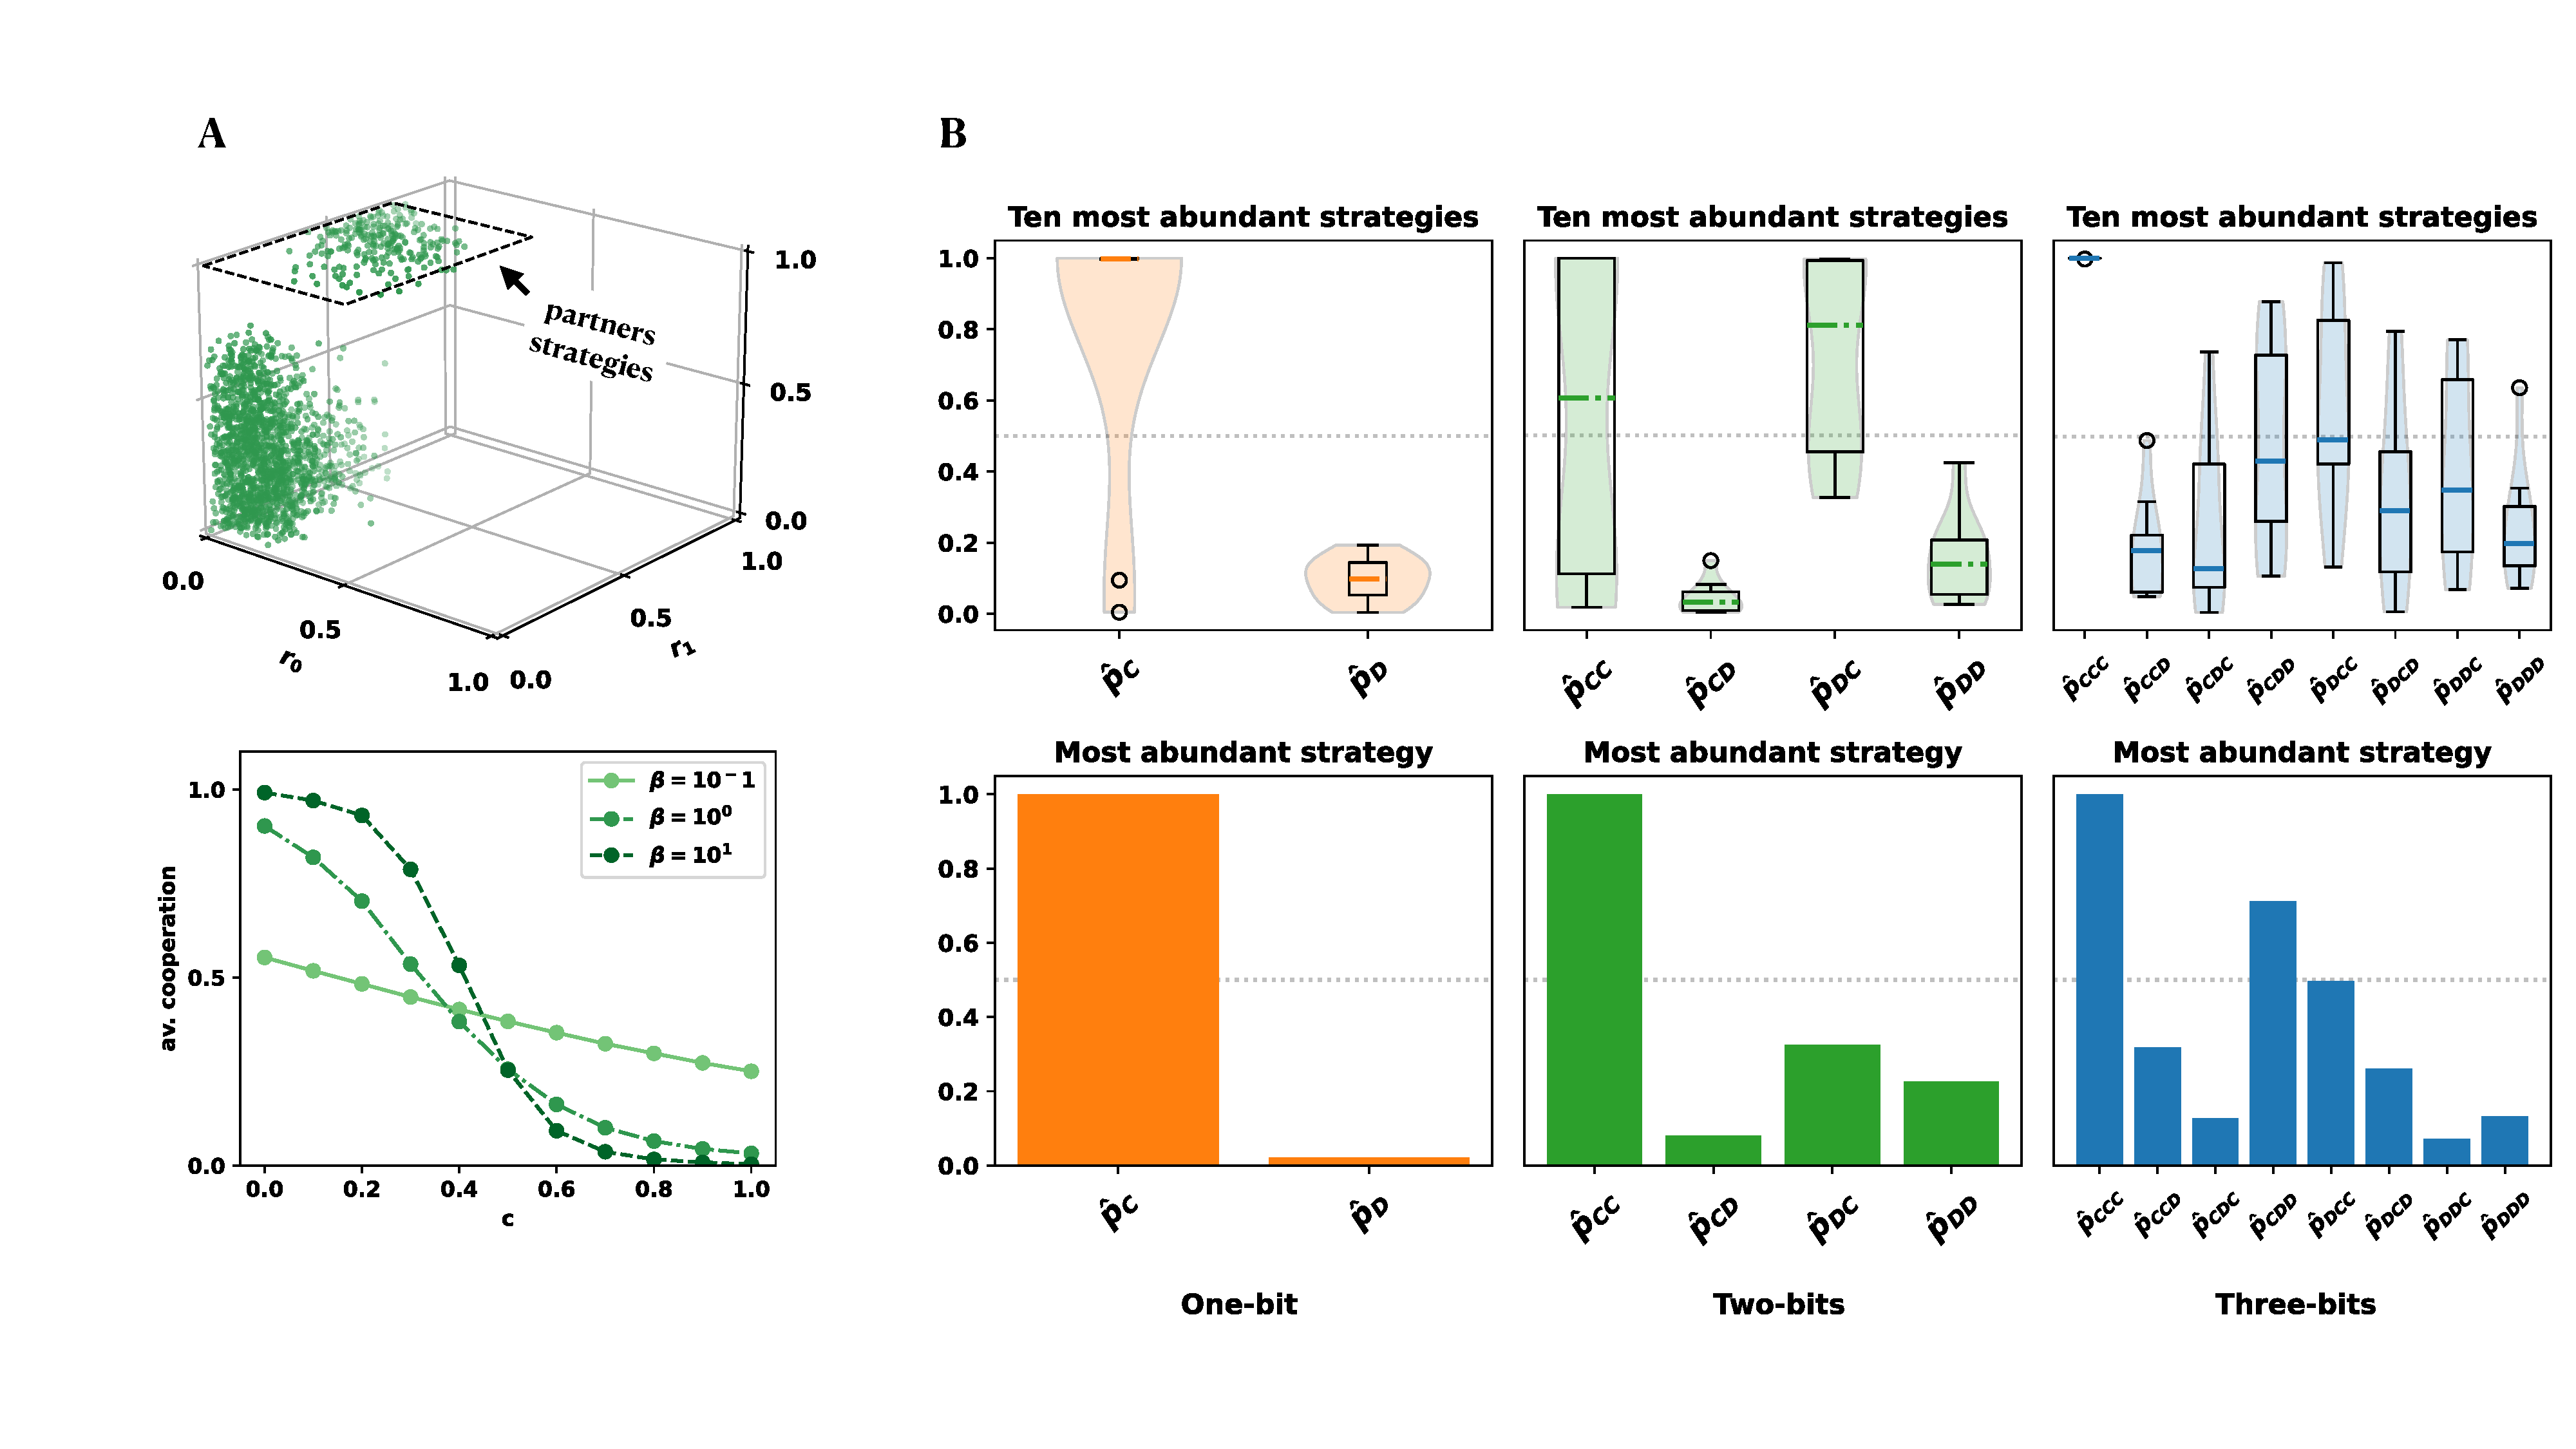
\includegraphics[width=\textwidth]{figures/evolutionary_dynamics_one_two_three.pdf}
  \caption{\textbf{Evolving strategies for $n=1, n=2$ and $n=3$.} In the previous sections we have
  characterized partners strategies for two and three bit reactive cases, and we
  have also discussed the case of counting reactive strategies. Here we want to
  assess whether partner strategies are strategies that evolve, thus are beneficial to
  adopt in an evolutionary setting. We ran simulations based on Imhof and Nowak.
  For a single run of the evolutionary process, we record the cooperating
  probabilities of the resident at each elementary time step. \textbf{A. Counting
  two-bit reactive strategies}. In the top panel we show the most abundant
  strategies of the evolutionary process when the population can use any
  counting two-bit reactive strategy ($r_0, r_1, r_2$). The abundant
  strategies are the residents that were fixed for the most time steps.
  The most abundant strategies fall within the region of the partner strategies.
  In the bottom panel we look at the evolving cooperation rate closer. The
  average cooperation is calculated by considering the cooperation rate within
  the resident population. For a given $\beta$ value we vary the cost $c \in [0, 1]$
  whilst we have fixed $b=1$. Three curves are shown, these are for different values
  of selection strength, $\beta \in {10^-1, 10^0, 10^1}$.
  \textbf{B. One, two, three bits.} We ran 10 independent simulations for each
  set of strategies and recorded the most abundant strategy for each run. The
  abundant strategy is the resident that was fixed for the most time steps. For
  the simulations we used \(b=1 \text{ and } c=.5\). For $n$ equal to 1 and
  2, \(T= 10 ^ 7\) and for $n=3$ then \(T= 2 \times10 ^ 7\).}
\end{figure}

\begin{figure}[h!]
  \centering
  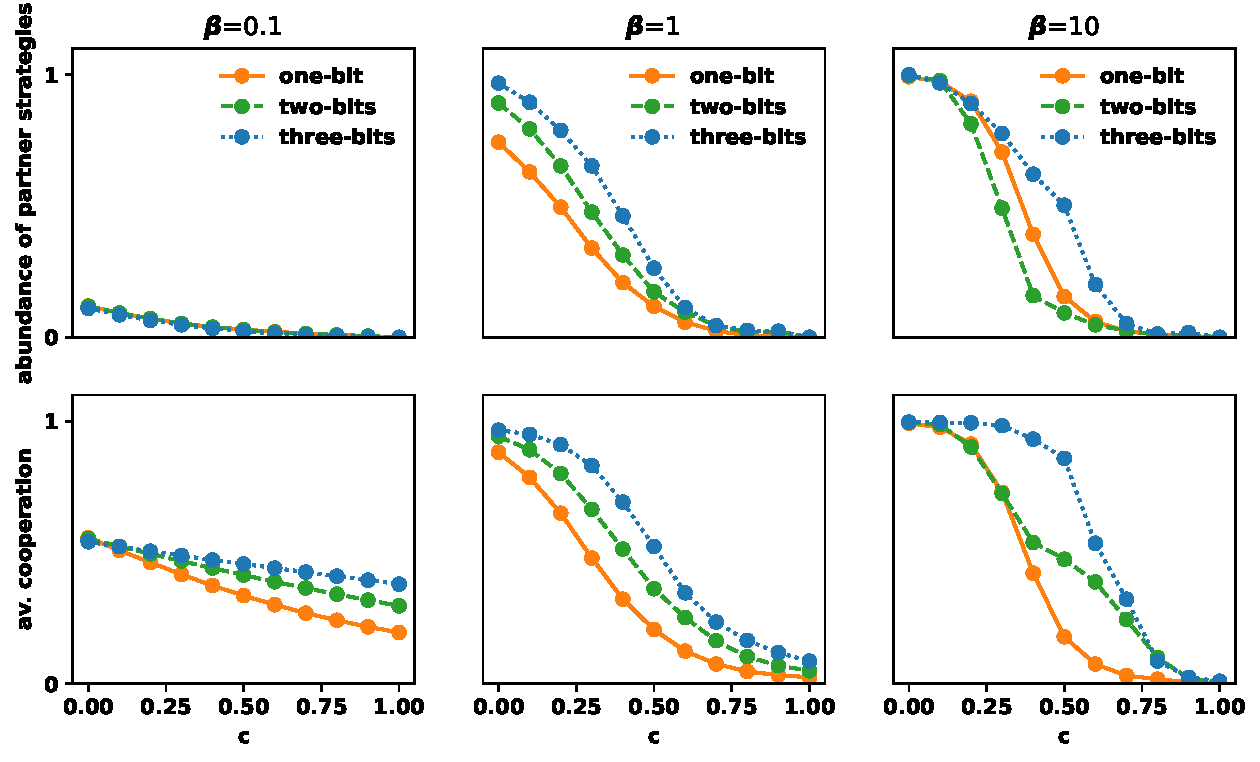
\includegraphics[width=\textwidth]{figures/abundance_of_partner_strategies.pdf}
  \caption{\textbf{Abundance of partner strategies.}
  We ran simulations based on Imhof and Nowak, varying the cost ($c$) and
  strength of selection ($\beta$). The cooperation benefit ($b$) is fixed at a
  value of 1. The results demonstrate that partner strategies evolve notably
  under strong selection ($\beta=1$) and lower cost conditions. Furthermore, the abundance
  of partner strategies is consistently higher when individuals have access to
  greater memory. The bottom panel displays how these partner strategies lead to
  increased levels of cooperation.}
\end{figure}

\section{Discussion}

~\\
\bibliography{bibliography.bib}

\end{document}